\chapter{Modelado y evaluación}

En este capítulo se detalla el modelado y evaluación llevado a cabo para resolver el problema de ciencia de datos propuesto y obtener un modelo de regresión final capaz de predecir el tiempo de diagnóstico de los pacientes.

En primer lugar se describe la \textbf{experimentación} a realizar - empezando por los modelos propuestos, los hiperparámetros planteados para cada uno de ellos y el proceso de \textbf{búsqueda} realizado para ajustarlos; y siguiendo con el proceso final de \textbf{selección de modelos} evaluando sobre un conjunto de datos separado. Tras esto, se muestran y estudian los \textbf{resultados} - tanto el rendimiento de los modelos y sus atributos como el comportamiento del modelo final elegido en comparación con el modelo ganador de la competición.

\section{Modelado y experimentación}

Tras el análisis exploratorio y el preprocesamiento del conjunto de datos realizado en los capítulos anteriores, la siguiente etapa del ciclo de vida de la ciencia de datos es el \textbf{modelado}: la propuesta de modelos de aprendizaje automático e hiperparámetros, el ajuste de éstos y el proceso de selección final para obtener un \textbf{modelo de regresión entrenado} capaz de resolver el problema propuesto con el menor error posible.

Para llevar a cabo este ajuste y selección es necesario realizar a la vez un proceso paralelo de \textbf{experimentación}, donde se evalua el rendimiento de todos los modelos bajo distintos parámetros y circunstancias, con el fin de seleccionar el mejor modelo de todos los propuestos.

\subsection{Modelos e hiperparámetros propuestos}

Se han propuesto un total de \textbf{16 modelos} para resolver el problema de la predicción del tiempo de diagnóstico de cáncer - correspondiéndose con los algoritmos estudiados durante la revisión de técnicas realizada en el Capítulo 2. Además, para cada uno de estos modelos se ha planteado una \textbf{malla de hiperparámetros} - un rango de posibles valores a ajustar para cada uno de los hiperparámetros.

Los modelos propuestos y sus mallas de hiperparámetros se describen a continuación agrupados según la \textbf{familia de modelos} a la que pertenecen - al compartir todos los modelos de una misma familia los mismos hiperparámetros a ajustar, salvo excepciones.

\subsubsection{Modelos de regresión lineal}

Los modelos de regresión lineal son la familia de algoritmos más sencilla utilizada, planteados para servir como \textbf{\textit{baselines}} - resultados a utilizar como punto de referencia para estudiar la mejora del error en algoritmos más complejos. Concretamente, se han planteado los siguientes modelos - siendo los hiperparámetros asociados los descritos en la \textbf{Tabla \ref{tab:ch5linealhyperparameters}}:

\begin{itemize}[parsep=1pt, itemsep=0pt, topsep=1pt]
	\item Regresión lineal simple.
	\item Regresión con regularización Ridge (L2).
	\item Regresión con regularización Lasso (L1).
	\item Regresión con \textit{Elastic-Net}.
\end{itemize}

\begin{table}[h]
	\vspace{-8mm}
	\centering
	\resizebox{0.9\textwidth}{!}{%
		\begin{tabular}{@{}rlll@{}}
			\toprule
			\multicolumn{1}{l}{\textbf{Hiperparámetro}} & \textbf{Rango}                      & \textbf{Descripción}                                                                                                                                                  & \textbf{Aplicable a}                                          \\ \midrule
			alfa                                        & $\{10^{-6}, 10^{-5}, \dots, 10^6\}$ & \begin{tabular}[c]{@{}l@{}}Factor de penalización aplicado a los parámetros.\\ Valores más altos implican una mayor penalización.\end{tabular}                        & \begin{tabular}[c]{@{}l@{}}L1, L2,\\ Elastic-Net\end{tabular} \\
			\rowcolor[HTML]{EFEFEF} 
			ratio                                       & $\{0.25, 0.5, 0.75\}$               & \begin{tabular}[c]{@{}l@{}}Ratio en el que se aplica la penalización de Lasso - L1.\\ 0 significa un modelo Ridge (L2), 1 significa un modelo Lasso (L1)\end{tabular} & Elastic-Net                                                   \\ \bottomrule
		\end{tabular}%
	}
	\captionsetup{belowskip=-40pt, justification=centering}
	\caption{Hiperparámetros planteados para modelos de regresión lineal}
	\label{tab:ch5linealhyperparameters}
\end{table}

\subsubsection{Árboles de decisión}

Solo se estudia un modelo de árbol, pudiendo observarse los hiperparámetros planteados en la \textbf{Tabla \ref{tab:ch5treehyperparameters}}.

\begin{table}[h]
	\vspace{-7mm}
	\centering
	\resizebox{0.9\textwidth}{!}{%
		\begin{tabular}{@{}rll@{}}
			\toprule
			\multicolumn{1}{l}{\textbf{Hiperparámetro}} &
			\textbf{Rango} &
			\textbf{Descripción} \\ \midrule
			max\_depth &
			$\{1, 2, \dots, 10, None\}$ &
			\begin{tabular}[c]{@{}l@{}}Profundidad máxima permitida para el crecimiento del árbol.\\ "None" indica que no se limita la profundidad.\end{tabular} \\
			\rowcolor[HTML]{EFEFEF} 
			min\_samples\_split &
			$\{2, 3, \dots, 50\}$ &
			\begin{tabular}[c]{@{}l@{}}Número mínimo de instancias requerido para particionar un nodo, \\ creando hojas a partir de éste.\end{tabular} \\
			min\_samples\_leaf &
			$\{1, 2, \dots, 50\}$ &
			\begin{tabular}[c]{@{}l@{}}Número mínimo de instancias en las hojas resultantes de una partición.\\ Un nodo no puede particionarse si alguna de las hojas resultantes \\ tiene un número menor de instancias.\end{tabular} \\
			\rowcolor[HTML]{EFEFEF} 
			criterion &
			\begin{tabular}[c]{@{}l@{}}$$\{"squared\_error",\\ "friedman\_mse",\\ "absolute\_error\}$$\end{tabular} &
			Función de error utilizada para elegir la partición más valiosa. \\ \bottomrule
		\end{tabular}%
	}
	\captionsetup{belowskip=-40pt, justification=centering}
	\caption{Hiperparámetros planteados para árboles de decisión}
	\label{tab:ch5treehyperparameters}
\end{table}

\subsubsection{Máquinas de vector de soporte}

Se han planteado \textbf{cuatro} modelos de máquinas de vector de soporte, según la \textbf{función kernel} utilizada - siendo los hiperparámetros asociados a dichas máquinas los descritos en la \textbf{Tabla \ref{tab:ch5svrhyperparameters}}.

\begin{itemize}[parsep=1pt, itemsep=0pt, topsep=1pt]
	\item Kernel lineal.
	\item Kernel polinómico.
	\item Kernel gaussiano.
	\item Kernel sigmoide.
\end{itemize}

\begin{table}[h]
	\vspace{-4mm}
	\centering
	\resizebox{0.9\textwidth}{!}{%
		\begin{tabular}{@{}rlll@{}}
			\toprule
			\multicolumn{1}{l}{\textbf{Hiperparámetro}} & \textbf{Rango}       & \textbf{Descripción}                                                                                                                                                                                                                     & \textbf{Aplicable a} \\ \midrule
			epsilon                                     & $[10^{-3}, 1]$      & \begin{tabular}[c]{@{}l@{}}Margen de error del hiperplano de máxima confianza.\\ Los puntos a una distancia menor a $\epsilon$ del hiperplano se predicen\\ con el valor del hiperplano directamente.\end{tabular}                       & Todos                \\
			\rowcolor[HTML]{EFEFEF} 
			tol                                         & $[10^{-7}, 1]$      & \begin{tabular}[c]{@{}l@{}}Tolerancia durante el entrenamiento.\\ Si la mejora en el error no es superior a $tol$, se detiene el entrenamiento.\end{tabular}                                                                             & Todos                \\
			C                                           & $[10^{-2}, 10^3]$   & \begin{tabular}[c]{@{}l@{}}Parámetro de regularización Ridge - L2 para penalizar pesos elevados.\\ La fuerza de regularización es inversamente proporcional a $C$ -\\ valores más bajos suponen regularizaciones más altas.\end{tabular} & Todos                \\
			\rowcolor[HTML]{EFEFEF} 
			degree                                      & $\{1, 2, \dots, 6\}$ & Grado del polinomio utilizado para definir el hiperplano.                                                                                                                                                                                & SVR polinómica       \\ \bottomrule
		\end{tabular}%
	}
	\captionsetup{belowskip=-40pt, justification=centering}
	\caption{Hiperparámetros planteados para máquinas de vector de soporte}
	\label{tab:ch5svrhyperparameters}
\end{table}

\subsubsection{Ensembles de Bagging}

Se han planteado \textbf{dos} \textit{ensembles} de tipo \textit{bagging}, utilizando \textbf{árboles de decisiones} como modelos sencillos a agrupar:

\begin{itemize}[parsep=1pt, itemsep=0pt, topsep=1pt]
	\item \textit{Random Forest}.
	\item \textit{Extremely Randomized Trees}.
\end{itemize}

Los hiperparámetros de los modelos se encuentran descritos en la \textbf{Tabla \ref{tab:ch5bagginghyperparameters}}:

\begin{table}[h]
	\vspace{-8mm}
	\centering
	\resizebox{0.9\textwidth}{!}{%
		\begin{tabular}{@{}rlll@{}}
			\toprule
			\textbf{Hiperparámetro} & \textbf{Rango}           & \textbf{Descripción}                                                     & \textbf{Aplicable a} \\ \midrule
			n\_estimators           & $\{50, 51, \dots, 200\}$ & Número de árboles a entrenar en el ensemble.                             & Todos                \\
			\rowcolor[HTML]{EFEFEF} 
			max\_features           & $[0.3, 1.0]$             & Porcentaje de atributos muestreados para el entrenamiento de cada árbol. & Todos                \\
			max\_depth              & $\{1, 2, \dots, 50\}$    & Profundidad máxima para cada árbol entrenado.                            & Todos                \\
			\rowcolor[HTML]{EFEFEF} 
			min\_samples\_split &
			$\{2, 3, \dots, 50\}$ &
			\begin{tabular}[c]{@{}l@{}}Número mínimo de instancias requerido para particionar un nodo\\ en cada árbol entrenado.\end{tabular} &
			Todos \\ \bottomrule
		\end{tabular}%
	}
	\captionsetup{belowskip=-40pt, justification=centering}
	\caption{Hiperparámetros planteados para ensembles de bagging}
	\label{tab:ch5bagginghyperparameters}
\end{table}

\subsubsection{Ensembles de Boosting}

Se ha planteado un único modelo de \textit{boosting} - \textbf{AdaBoost} -, utilizando \textbf{árboles de decisiones} como modelo sencillo a agrupar. Sus hiperparámetros se encuentran descritos en la \textbf{Tabla \ref{tab:ch5boostinghyperparameters}}.

\begin{table}[h]
	\vspace{-8mm}
	\centering
	\resizebox{0.9\textwidth}{!}{%
		\begin{tabular}{@{}rll@{}}
			\toprule
			\textbf{Hiperparámetro} &
			\textbf{Rango} &
			\textbf{Descripción} \\ \midrule
			n\_estimators &
			$\{50, 51, \dots, 200\}$ &
			Número de árboles a entrenar en el ensemble. \\
			\rowcolor[HTML]{EFEFEF} 
			learning\_rate &
			$[10^{-4}, 10]$ &
			\begin{tabular}[c]{@{}l@{}}Ponderación aplicada a cada modelo nuevo.\\ En general, representa la velocidad de aprendizaje del modelo, donde\\ valores altos implican cambios más rápidos de los pesos.\end{tabular} \\ \bottomrule
		\end{tabular}%
	}
	\captionsetup{belowskip=-40pt, justification=centering}
	\caption{Hiperparámetros planteados para ensembles de boosting}
	\label{tab:ch5boostinghyperparameters}
\end{table}

\subsubsection{Ensembles de Gradient Boosting}

Se han planteado \textbf{cuatro} ensembles con la técnica de \textit{Gradient Boosting}, utilizando \textbf{árboles de decisiones} como modelos sencillos a agrupar - siendo sus hiperparámetros comunes los descritos en la \textbf{Tabla \ref{tab:ch5gboostcommon}}.

\begin{itemize}[parsep=1pt, itemsep=0pt, topsep=1pt]
	\item \textit{eXtreme Gradient Boosting}.
	\item \textit{Categorical Boosting}.
	\item \textit{Light Gradient Boosting Machine}.
	\item \textit{Histogram Based Gradient Boosting}.
\end{itemize}

\begin{table}[h]
	\vspace{-4mm}
	\centering
	\resizebox{0.9\textwidth}{!}{%
		\begin{tabular}{rll}
			\hline
			\multicolumn{1}{l}{\textbf{Hiperparámetro}}                     & \textbf{Rango}           & \textbf{Descripción}                          \\ \hline
			\begin{tabular}[c]{@{}r@{}}Número de\\ estimadores\end{tabular} & $\{50, 51, \dots, 200\}$ & Número de árboles a entrenar en el ensemble.  \\
			\rowcolor[HTML]{EFEFEF} 
			\begin{tabular}[c]{@{}r@{}}Profundidad\\ máxima\end{tabular}    & $\{1, 2, \dots, 10\}]$   & Profundidad máxima para cada arbol entrenado. \\
			\begin{tabular}[c]{@{}r@{}}Tasa de\\ aprendizaje\end{tabular} &
			$[0.01, 1.0]$ &
			\begin{tabular}[c]{@{}l@{}}Ponderación aplicada a cada modelo nuevo.\\ Velocidad de aprendizaje del modelo, donde valores altos\\ implican cambios más rápidos en los pesos.\end{tabular} \\ \hline
		\end{tabular}%
	}
	\captionsetup{belowskip=-20pt, justification=centering}
	\caption{Hiperparámetros comunes a los modelos de Gradient Boosting}
	\label{tab:ch5gboostcommon}
\end{table}

A diferencia del resto de modelos propuestos, estos modelos tienen algunas peculiaridades: 
\begin{itemize}[parsep=1pt, itemsep=1pt, topsep=2pt]
	\item \textbf{Librerías externas:} A diferencia del resto de modelos - trabajando siempre con implementaciones de \textit{scikit-learn} -, los modelos de \textit{Gradient Boosting} están disponibles a través de librerías independientes. Esto se traduce en que \textbf{presentan hiperparámetros y ajustes distintos entre sí}.
	\item \textbf{GPU:} Las implementaciones de estos modelos están diseñadas para agilizar el entrenamiento a través de una \textbf{tarjeta gráfica} - lo que puede llegar a hacerlos más rápidos que otros modelos más simples.
	\item \textbf{Atributos categóricos:} Los modelos de \textit{Gradient Boosting} trabajan de forma autónoma con atributos categóricos, por lo que \textbf{no es necesario realizar codificación}.
\end{itemize}

Debido a estas diferencias, es necesario realizar algunos ajustes adicionales de hiperparámetros específicos para cada modelo. Estos hiperparámetros adicionales quedan descritos en la \textbf{Tabla \ref{tab:ch5gboostspecific}}.

\begin{table}[h]
	\vspace{-6mm}
	\centering
	\resizebox{0.9\textwidth}{!}{%
		\begin{tabular}{rlll}
			\hline
			\multicolumn{1}{l}{\textbf{Hiperparámetro}}                                    & \textbf{Rango}           & \textbf{Descripción}                                                                                                                               & \textbf{Modelo}                                                      \\ \hline
			Profundidad máxima                                                             & $\{4, 5, \dots, 10\}$    & Profundidad máxima para cada árbol entrenado.                                                                                                      & XGBoost                                                              \\
			\rowcolor[HTML]{EFEFEF} 
			Umbral de mejora                                                               & $[0, 10^4]$              & \begin{tabular}[c]{@{}l@{}}Error mínimo a reducir para considerar la partición\\ de un nodo.\end{tabular}                                          & XGBoost                                                              \\
			Porcentaje de instancias                                                       & $[0.3, 1.0]$             & Porcentaje de instancias del conjunto de datos muestreadas.                                                                                        & XGBoost                                                              \\
			\rowcolor[HTML]{EFEFEF} 
			Porcentaje de atributos                                                        & $[0.3, 1.0]$             & Porcentaje de atributos del conjunto de datos muestreados.                                                                                         & \begin{tabular}[c]{@{}l@{}}XGBoost,\\ HistGradientBoost\end{tabular} \\ \hline
			Regularización                                                                 & $[10^{-3}, 10]$          & \begin{tabular}[c]{@{}l@{}}Coeficiente aplicado a la regularización de tipo Ridge (L2)\\ para penalizar ensembles con pesos elevados.\end{tabular} & CatBoost                                                             \\
			\rowcolor[HTML]{EFEFEF} 
			\begin{tabular}[c]{@{}r@{}}Intensidad de\\ la aleatoriedad\end{tabular}        & $[1, 2]$                 & \begin{tabular}[c]{@{}l@{}}Multiplicador aplicado a la varianza de cada posible partición\\ para forzar aleatoriedad.\end{tabular}                 & CatBoost                                                             \\ \hline
			\begin{tabular}[c]{@{}r@{}}Número máximo de\\ hojas\end{tabular}               & $\{10, 11, \dots, 100\}$ & \begin{tabular}[c]{@{}l@{}}Número máximo de hojas que puede tener cada árbol -\\ independientemente de su profundidad.\end{tabular}                & \begin{tabular}[c]{@{}l@{}}LGBM,\\ HistGradientBoost\end{tabular}    \\
			\rowcolor[HTML]{EFEFEF} 
			\begin{tabular}[c]{@{}r@{}}Número mínimo de\\ instancias por hoja\end{tabular} & $\{20, 21, \dots, 200\}$  & \begin{tabular}[c]{@{}l@{}}Número mínimo de instancias en las hojas resultantes de\\ una partición.\end{tabular}                                   & \begin{tabular}[c]{@{}l@{}}LGBM,\\ HistGradientBoost\end{tabular}    \\ \hline
	\end{tabular}%
}
\captionsetup{belowskip=-40pt, justification=centering}
\caption{Hiperparámetros específicos para modelos de Gradient Boosting}
\label{tab:ch5gboostspecific}
\end{table}

\subsection{Experimentación}

Tras la definición de modelos, el siguiente paso es definir la \textbf{experimentación} a realizar: el proceso guiado de búsqueda a través del cual se realiza el \textbf{ajuste de hiperparámetros} y \textbf{selección de atributos} para cada modelo y la \textbf{selección del modelo final} para resolver el problema de regresión.

En todos los casos, la selección se hace con el objetivo de \textbf{minimizar el error del modelo} - es decir, se eligen los hiperparámetros y el modelo que llevan al menor error posible de todas las opciones. Para todos los experimentos, la métrica de error utilizada es la \textbf{raíz del error cuadrático medio (\textit{RMSE})}, siguiendo la fórmula:

$$\text{RMSE} = \sqrt{\frac{1}{N} \sum_{n=1}^{N}\left( y^{(n)} - \hat{y}^{(n)}\right)^2}$$

Donde $y^{(n)}$ es el valor esperado y $\hat{y}^{(n)}$ es el valor predicho para la instancia $n$ del conjunto de datos.

Para realizar los experimentos se cuentan con los siguientes \textbf{conjuntos de datos}, cuyo uso será descrito en las secciones posteriores:
\begin{itemize}[parsep=1pt, itemsep=1pt, topsep=4pt]
	\item \textbf{Conjunto de entrenamiento:} 9879 instancias, obtenido a partir del $75\%$ del conjunto de datos inicial.
	\item \textbf{Conjunto de validación:} 3294 instancias, obtenido a partir del $25\%$ del conjunto de datos inicial.
	\item \textbf{Conjunto de test:} 5646 instancias, ofrecido por separado al conjunto de datos inicial. \textbf{No se tienen los valores esperados para el tiempo de diagnóstico} - teniendo que evaluarse el error a través de una plataforma externa.
\end{itemize}

\subsubsection{Ajuste de hiperparámetros}

La primera fase de experimentación es el \textbf{ajuste de hiperparámetros:} la selección, para cada modelo propuesto, tanto de los \textbf{hiperparámetros} como del \textbf{subconjunto de atributos} que minimizan el error final del modelo. 

Dicho ajuste se realiza a través de una \textbf{selección de hiperparámetros con validación cruzada} - se entrena un modelo para cada par de hiperparámetros y subconjunto de atributos sobre el conjunto de entrenamiento utilizando \textbf{validación cruzada de 5-folds} para obtener un error promedio honesto. Ahora bien, como se ha visto en la sección anterior, \textbf{el número de posibles hiperparámetros para cada modelo puede resultar excesivo} - lo cual, mezclado con el tiempo de entrenamiento de los modelos más complejos, puede hacer la evaluación de todas las combinaciones de hiperparámetros en un tiempo razonable imposible. 

Para solucionar este problema se plantean varias metodologías de \textbf{búsqueda de hiperparámetros} - es decir, distintas estrategias para determinar \textbf{cuáles de todos los posibles conjuntos de hiperparámetros propuestos se evalúan}:
\begin{itemize}[parsep=2pt, itemsep=2pt, topsep=4pt]
	\item \textbf{Búsqueda exhaustiva:} Se prueban \textbf{todas las posibles combinaciones de hiperparámetros}. Si bien ofrece la garantía de encontrar una solución óptima, también acarrea un coste exponencial que deja de ser factible para modelos complejos.
	
	\item \textbf{Búsqueda aleatoria uniforme:} Para evitar una búsqueda exhaustiva, la primera opción es realizar en su lugar una \textbf{búsqueda totalmente aleatoria}, evaluando un número fijo de combinaciones aleatorias para seleccionar el mejor. Si bien es sustancialmente más rápido y suele dar resultados aceptables para un número suficiente de búsquedas, se pierde la garantía de encontrar una solución óptima.
	
	Para los modelos propuestos, se ha elegido de forma empírica evaluar \textbf{100 conjuntos de hiperparámetros aleatorios}.
	
	\item \textbf{Búsqueda aleatoria gaussiana:} La búsqueda aleatoria uniforme puede tener problemas al trabajar con modelos muy complejos con tiempos largo de entrenamiento, al tener que probar un gran número de hiperparámetros para encontrar un modelo razonable. Una solución a este algoritmo es guiar las búsquedas aleatorias con un modelo \textbf{probabilístico} - donde los hiperparámetros con menor error son más probables. De esta forma se puede reducir el número necesario de conjuntos de hiperparámetros evaluados para obtener un buen resultado. 
	
	Para los modelos propuestos, se ha elegido de forma empírica evaluar \textbf{50 conjuntos de hiperparámetros aleatorios}.
\end{itemize}

\begin{table}[h]
	\vspace{-6mm}
	\centering
	\resizebox{\textwidth}{!}{%
		\begin{tabular}{@{}rrrrrrrrrrrrrrrrr@{}}
			\toprule
			\multicolumn{1}{l}{} &
			\multicolumn{1}{c}{\textbf{\begin{tabular}[c]{@{}c@{}}Regresión \\ Lineal\end{tabular}}} &
			\multicolumn{1}{c}{\textbf{\begin{tabular}[c]{@{}c@{}}Ridge \\ L2\end{tabular}}} &
			\multicolumn{1}{c}{\textbf{\begin{tabular}[c]{@{}c@{}}Lasso \\ L1\end{tabular}}} &
			\multicolumn{1}{c}{\textbf{\begin{tabular}[c]{@{}c@{}}Elastic-\\ Net\end{tabular}}} &
			\multicolumn{1}{c}{\textbf{\begin{tabular}[c]{@{}c@{}}Árbol de \\ decisión\end{tabular}}} &
			\multicolumn{1}{c}{\textbf{\begin{tabular}[c]{@{}c@{}}SVR\\ Lineal\end{tabular}}} &
			\multicolumn{1}{c}{\textbf{\begin{tabular}[c]{@{}c@{}}SVR\\ Polinomica\end{tabular}}} &
			\multicolumn{1}{c}{\textbf{\begin{tabular}[c]{@{}c@{}}SVR\\ Gaussiana\end{tabular}}} &
			\multicolumn{1}{c}{\textbf{\begin{tabular}[c]{@{}c@{}}SVR\\ Sigmoide\end{tabular}}} &
			\multicolumn{1}{c}{\textbf{\begin{tabular}[c]{@{}c@{}}Random\\ Forest\end{tabular}}} &
			\multicolumn{1}{c}{\textbf{\begin{tabular}[c]{@{}c@{}}Extremely\\ Random Trees\end{tabular}}} &
			\multicolumn{1}{c}{\textbf{\begin{tabular}[c]{@{}c@{}}Ada\\ Boost\end{tabular}}} &
			\multicolumn{1}{c}{\textbf{XGBoost}} &
			\multicolumn{1}{c}{\textbf{CatBoost}} &
			\multicolumn{1}{c}{\textbf{LGBM}} &
			\multicolumn{1}{c}{\textbf{\begin{tabular}[c]{@{}c@{}}HistGradient\\ Boost\end{tabular}}} \\ \midrule
			\textbf{\begin{tabular}[c]{@{}r@{}}Tipo de\\ búsqueda\end{tabular}} &
			Exhaustiva &
			Exhaustiva &
			Exhaustiva &
			Exhaustiva &
			Aleatoria &
			Aleatoria &
			Aleatoria &
			Aleatoria &
			Aleatoria &
			Gaussiana &
			Gaussiana &
			Gaussiana &
			Gaussiana &
			Gaussiana &
			Gaussiana &
			Gaussiana \\
			\rowcolor[HTML]{EFEFEF} 
			\textbf{\begin{tabular}[c]{@{}r@{}}Conjuntos\\ estudiados\end{tabular}} &
			7 &
			91 &
			91 &
			273 &
			100 &
			100 &
			100 &
			100 &
			100 &
			50 &
			50 &
			50 &
			50 &
			50 &
			50 &
			50 \\
			\rowcolor[HTML]{FFFFFF} 
			\textbf{\begin{tabular}[c]{@{}r@{}}Modelos\\ totales\\ entrenados\end{tabular}} &
			140 &
			1820 &
			1820 &
			5460 &
			2000 &
			2000 &
			2000 &
			2000 &
			2000 &
			1000 &
			1000 &
			1000 &
			1000 &
			1000 &
			1000 &
			1000 \\ \bottomrule
		\end{tabular}%
	}
	\captionsetup{belowskip=-20pt, justification=centering}
	\caption{Número total de conjuntos de hiperparámetros y modelos entrenados para cada modelo.}
	\label{tab:ch5iteraciones}
\end{table}

En la \textbf{Tabla \ref{tab:ch5iteraciones}} se encuentra detallado el \textbf{número total de modelos entrenados} para cada modelo en base al tipo de búsqueda realizado, siguiendo el siguiente orden:
\begin{enumerate}[parsep=2pt, itemsep=2pt, topsep=4pt]
	\item \textbf{Subconjunto de atributos:} Uno de los hiperparámetros a elegir para cada modelo es el \textbf{subconjunto de atributos utilizado} - optando entre los tres subconjuntos propuestos o el conjunto de atributos completo. Por tanto, es necesario realizar la búsqueda \textbf{4 veces} para cada modelo.
	\item \textbf{Ajuste de hiperparámetros:} Dependiendo del tipo de búsqueda realizado, el número de conjuntos de hiperparámetros a evaluar cambia. Hay que destacar que un hiperparámetro a ajustar por todos los modelos es el \textbf{agrupamiento de valores durante la codificación} - siendo especialmente significativo en la búsqueda exhaustiva, donde crece el número de conjuntos a evaluar.
	\item \textbf{Validación cruzada:} Para cada par de subconjuntos de atributos e hiperparámetros se realiza una \textbf{5-validación cruzada} entrenando sobre el \textbf{conjunto de entrenamiento}, por lo que se entrenan cinco modelos y se obtiene el error promedio de éstos.
\end{enumerate}

Tras todos los modelos entrenados y evaluados, se elige para cada algoritmo \textbf{un único modelo final} - aquel que minimiza el error - para ser considerado durante la selección de modelos.

\subsubsection{Selección de modelos}

Tras el paso anterior de ajuste de hiperparámetros se ha obtenido un total de \textbf{16 modelos ajustados y entrenados} - uno por cada algoritmo considerado. El objetivo de la siguiente y última fase de la experimentación, por tanto, es la \textbf{selección del modelo final} - elegir el modelo con menor error \textbf{generalizable} a datos no conocidos previamente.

Con el fin de obtener una evaluación \textbf{honesta} del rendimiento de cada modelo, cada uno de estos modelos entrenados es evaluado sobre el \textbf{conjunto de validación} - un conjunto de datos al que no han tenido acceso hasta este momento.

El modelo final seleccionado es aquel que presenta el \textbf{menor error sobre el conjunto de validación}, siendo el modelo que se utilizará para resolver el problema de predicción de tiempo de diagnóstico de cáncer de metástasis, y cuyo rendimiento real se evaluará sobre el \textbf{conjunto de test}.

\section{Evaluación}

Tras el modelado y experimentación, el siguiente paso del ciclo de ciencia de datos es la \textbf{evaluación:} el estudio del \textbf{rendimiento real del modelo seleccionado}, para determinar si es capaz de resolver el problema propuesto - la predicción del tiempo de diagnóstico - con un \textbf{error aceptable}.

Además de este estudio del modelo final, resulta de interés académico estudiar el \textbf{rendimiento} de los modelos entrenados durante la experimentación estudiando estadísticos como el \textbf{error} o el \textbf{tiempo de entrenamiento} durante las fases de ajuste de hiperparámetros y selección de modelos.

\subsection{Rendimiento durante el ajuste de hiperparámetros}

El primer paso de la evaluación consiste en estudiar los resultados del ajuste de hiperparámetros - concretamente observar el \textbf{error y tiempo de entrenamiento} de los modelos, y estudiar como puede influir en éste los \textbf{subconjuntos de atributos}.

Los resultados completos de la fase de ajuste de hiperparámetros están disponibles en la \textbf{Tabla \ref{tab:annextrainingresults}} - realizándose el siguiente estudio a partir de gráficas.

\subsubsection{Error de los modelos durante el ajuste}

La \textbf{Figura \ref{fig:ch5trainerror}} representa la distribución del \textbf{menor error} para cada par de modelo y subconjunto de atributos - donde un menor error representa un \textbf{mejor modelo} - incluyendo, además, los \textbf{valores promedios} de cada subconjunto de atributos a través de lineas discontinuas. A partir de esta figura, se pueden realizar las siguientes observaciones:

\begin{figure}[h]
	\vspace{-4mm}
	\centering
	\makebox[\textwidth][c]{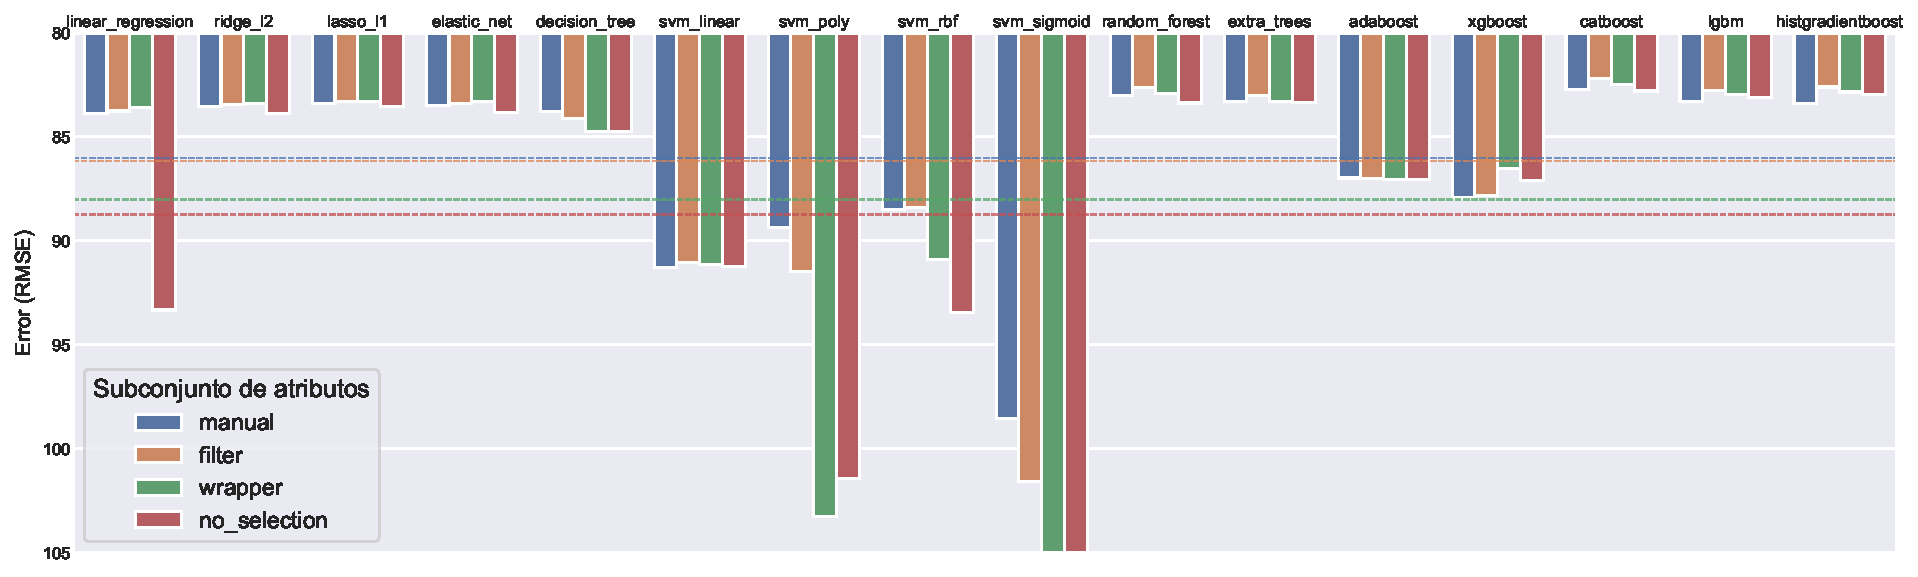
\includegraphics[width=1\linewidth]{figs/chapter5/training/error}}
	\captionsetup{aboveskip=-4pt, justification=centering}
	\caption{Error promedio durante el entrenamiento para cada modelo y subconjunto de atributos (acotado en un error máximo de 105)}
	\label{fig:ch5trainerror}
\end{figure}

\begin{itemize}[leftmargin=*, parsep=1pt, itemsep=0pt, topsep=1pt]
	\item En general, \textbf{todos los modelos presentan errores similares y elevados} - en el rango de $82-84$ unidades de error -, habiendo cierta variación dependiendo del subconjunto de atributos. También se cumple, como se esperaba, que \textbf{el error se reduce con la complejidad de los modelos}. Ahora bien, hay unos modelos comportándose como \textit{outliers}:
	\begin{itemize}[parsep=1pt, itemsep=0pt, topsep=1pt]
		\item \textbf{Máquinas de vector de soporte:} En todas las ocasiones las máquinas de vector de soporte ofrecen errores sustancialmente peores al del resto de modelos, siendo especialmente significativo para las \textbf{máquinas sigmoides}.
		\item \textbf{\textit{AdaBoost y XGBoost}:} A pesar de ser modelos complejos - \textit{ensembles} de \textit{Boosting} y \textit{Gradient Boosting} respectivamente -, sus errores son mayores al promedio del resto de modelos.
	\end{itemize}
	\item Se pueden observar \textbf{tres agrupamientos de subconjuntos de atributos}, con promedios de error similares:
	\begin{itemize}[parsep=1pt, itemsep=0pt, topsep=1pt]
		\item \textbf{Manual y Filter}: Los subconjuntos con menor error promedio, ambos presentan comportamientos y atributos muy similares - siendo la principal diferencia que \textit{filter} añade información numérica y ofrece ligeramente mejores resultados, especialmente en modelos \textbf{complejos} como \textit{ensembles}.
		
		\item \textbf{Wrapper}: Un subconjunto con menos atributos categóricos y más atributos numéricos, parece ofrecer los mejores resultados en los modelos de regresión lineal - los más simples y susceptibles a la alta dimensionalidad que introducen los atributos categóricos.
		
		\item \textbf{Conjunto completo:} Como era de esperar, el error tiende a ser mayor utilizando el conjunto completo de 150 atributos - presentando picos sustanciales en algunos modelos .
	\end{itemize}
	
	Es importante destacar que los promedios están \textbf{sesgados} por los errores elevados de las máquinas de vectores de soporte - lo que puede influir en que sean más elevados de lo que serían realmente.
\end{itemize}

\subsubsection{Tiempo de entrenamiento de los modelos durante el ajuste}

La \textbf{Figura \ref{fig:ch5traintime}} representa el \textbf{tiempo de entrenamiento} para el modelo entrenado, para cada par de modelo y subconjunto de atributos. A partir de esta figura, se pueden realizar las siguientes observaciones:

\begin{itemize}[leftmargin=*, parsep=2pt, itemsep=4pt, topsep=1pt]
	\item Como era de esperar, \textbf{la dimensionalidad del conjunto de datos aumenta el tiempo de entrenamiento} - los subconjuntos de atributos reducidos son, por lo general, sustancialmente más rápidos que los modelos entrenados sobre el conjunto de datos completo.
	
	Dentro de los subconjuntos, en general \textit{Filter} y \textit{Wrapper} son más lentos, al tener \textbf{10 atributos} frente a los \textbf{5} de \textit{Manual}. Ahora bien, en algunos modelos parece ser más rápido \textit{Wrapper}, posiblemente por el menor número de atributos categóricos.
	
	\item Por lo general, \textbf{la complejidad del modelo influye en el tiempo de entrenamiento} - con los modelos tradicionales más simples necesitando menos tiempo que los \textit{ensembles.}
	
	Las únicas excepciones se encuentran en las \textbf{máquinas de vectores de soporte} - que requieren un gran tiempo para aplicar funciones kernel complejas - y los \textbf{\textit{ensembles de Gradient Boosting}} - que, en contra de lo que se podría esperar por su gran complejidad, son de los modelos más rápidos al utilizar una GPU para paralelizar su entrenamiento.
\end{itemize}

\begin{figure}[h]
	\vspace{-6mm}
	\centering
	\makebox[\textwidth][c]{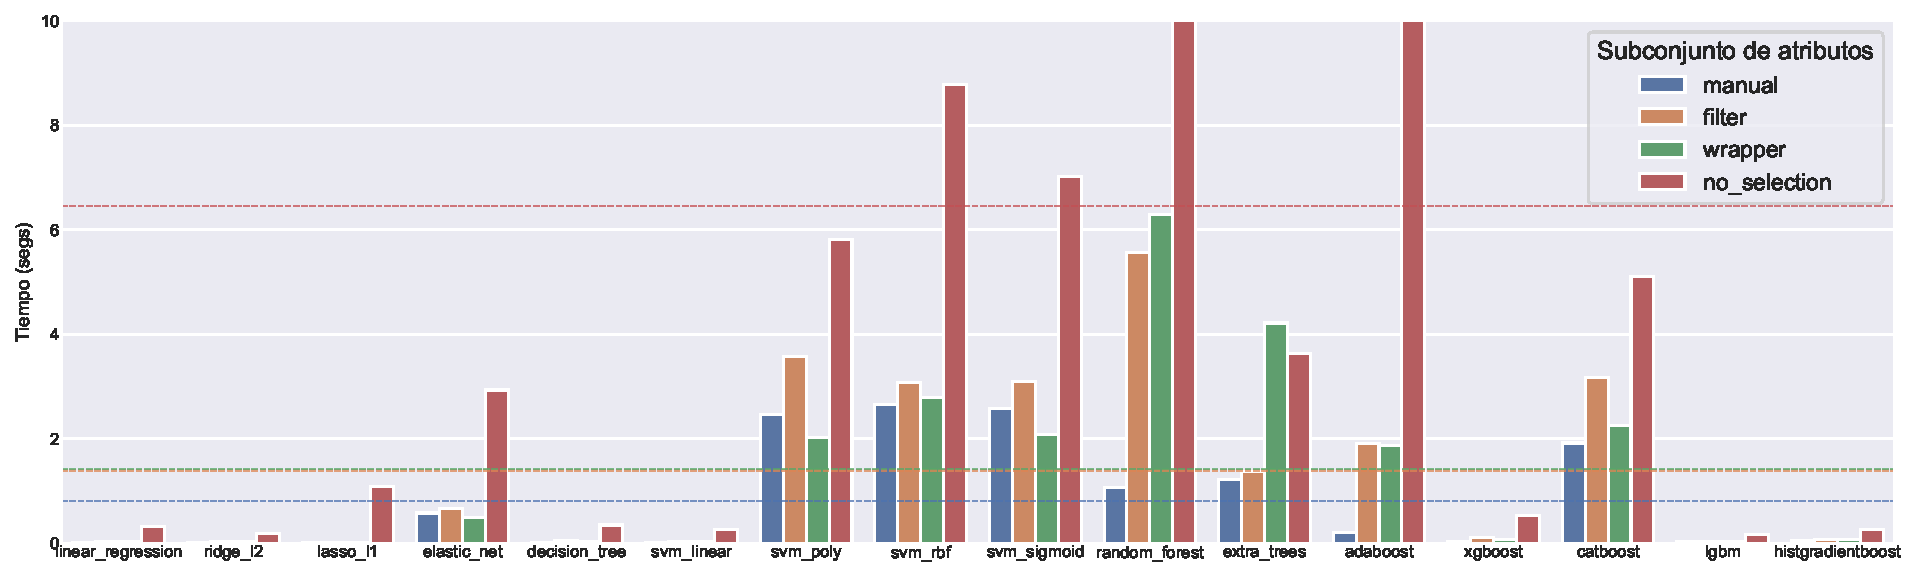
\includegraphics[width=1\linewidth]{figs/chapter5/training/time}}
	\captionsetup{belowskip=-40pt, justification=centering}
	\caption{Tiempo promedio de entrenamiento para cada modelo y subconjunto de atributos (acotado en 10 segundos)}
	\label{fig:ch5traintime}
\end{figure}

\subsection{Rendimiento durante la selección de modelos}

Tras el estudio del rendimiento durante el ajuste, el siguiente paso consiste en analizar el rendimiento de los \textbf{modelos entrenados} - concretamente estudiar los \textbf{subconjuntos de atributos seleccionados} y los \textbf{errores finales de los modelos sobre el conjunto de validación}.

Los resultados completos de la fase de selección de modelo están disponibles en la \textbf{Tabla \ref{tab:annexvalidation}} - realizándose el siguiente estudio a partir de gráficas.

\subsubsection{Subconjuntos de hiperparámetros utilizados}

En la \textbf{Figura \ref{fig:ch5featuresubsets}} se representa la distribución de los subconjuntos de atributos seleccionados durante el ajuste de hiperparámetros. Se pueden observar las siguientes características en el comportamiento:

\begin{figure}[h]
	\vspace{-8mm}
	\begin{center}
		\begin{subfigure}{0.35\linewidth}
			\begin{center}
				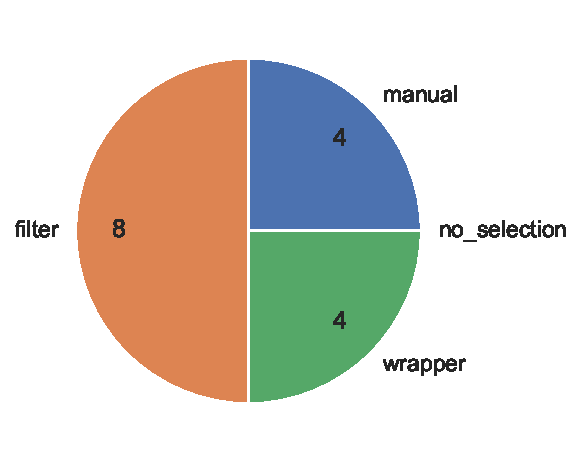
\includegraphics[width=\linewidth]{figs/chapter5/validation/fsfrequency}
				\caption{General}\label{fig:ch5fsgeneral}
			\end{center}
		\end{subfigure} 
		\begin{subfigure}{0.60\linewidth}
			\begin{center}
				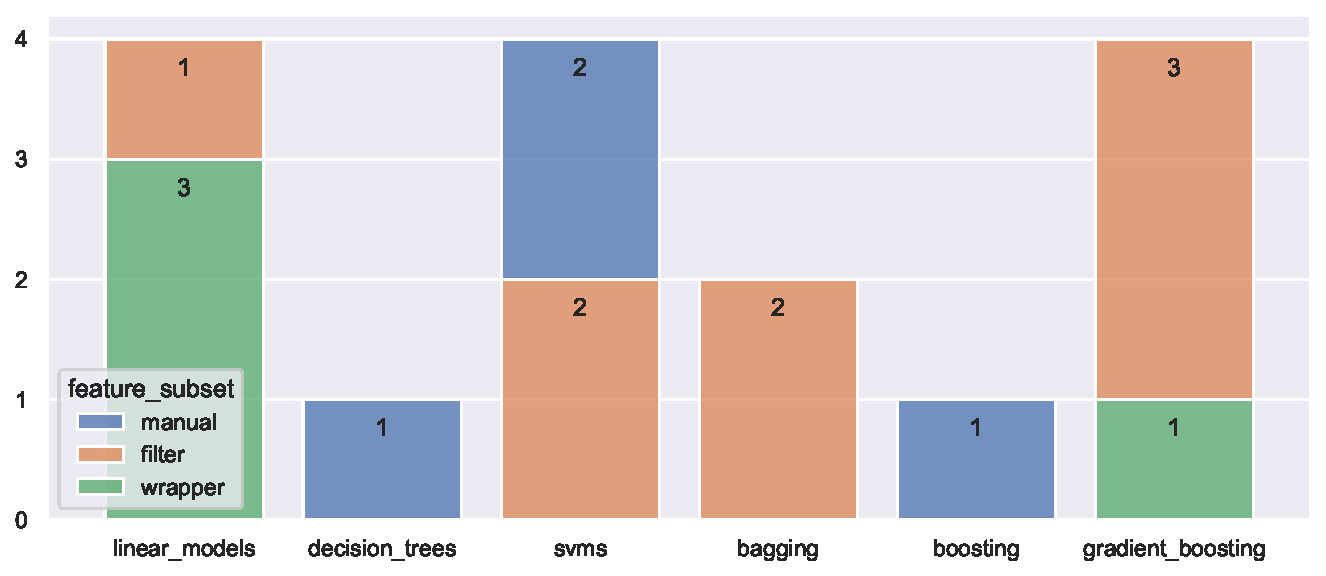
\includegraphics[width=\linewidth]{figs/chapter5/validation/fsfamily}
				\caption{Agrupado por familias}\label{fig:ch5fsfamily}
			\end{center}
		\end{subfigure} 
	\end{center}
	\captionsetup{aboveskip=-5pt, belowskip=-25pt}
	\caption{Distribución de los subconjuntos de atributos seleccionados}
	\label{fig:ch5featuresubsets}
\end{figure}

\begin{itemize}[leftmargin=*, parsep=1pt, itemsep=2pt, topsep=1pt]
	\item Los modelos tienden a utilizar subconjuntos con \textbf{atributos numéricos} - \textit{Filter y Wrapper} frente a \textit{Manual}. En contra de lo que se podría haber deducido a partir del análisis exploratorio, los \textbf{atributos numéricos aportan información util al modelo}. Concretamente:
	\begin{itemize}[parsep=1pt, itemsep=2pt, topsep=1pt]
		\item Los \textbf{modelos lineales} suelen utilizar \textit{Wrapper}, un subconjunto con menos atributos categóricos.
		\item Los \textbf{árboles de decisiones} y \textbf{máquinas de vector de soporte} utilizan \textit{Manual} con mayor frecuencia - posiblemente influyendo el ser el subconjunto más pequeño.
		\item Los \textit{\textbf{ensembles}}, más complejos, tienden a preferir \textit{Filter} - un subconjunto con la misma información categórica que \textit{Manual} pero información numérica adicional.
	\end{itemize}
	\item \textbf{Ningún modelo utiliza el conjunto de atributos completo} - por lo que se puede afirmar que la selección de atributos ha mejorado el rendimiento.
\end{itemize}

\subsubsection{Error de los modelos seleccionados}

La \textbf{Figura \ref{fig:ch5valerror}} representa el error sobre el \textbf{conjunto de validación} de cada modelo de regresión entrenado - ordenados de \textbf{menor a mayor error}. A partir de dicha gráfica, se pueden extraer las siguientes conclusiones:

\begin{itemize}[leftmargin=*, parsep=1pt, itemsep=2pt, topsep=1pt]
	\item \textbf{El error generalizado de los modelos es muy elevado:} Incluso para el mejor modelo - \textit{Categorical Boost}, con un error de \textbf{81.61} - el error es muy elevado si se tiene en cuenta que el rango de la variable objetivo en el conjunto de entrenamiento es aproximadamente $[0, 365]$.
	
	Al ser este error generalizado, lo más factible es asumir que \textbf{el conjunto de datos no tiene suficiente información para predecir esta información}.
	\item \textbf{Como era de esperar, los \textit{ensembles} ofrecen mejor rendimiento:} Los modelos con mejor rendimiento son los \textit{ensembles} - concretamente \textbf{Gradient Boosting} seguido de \textbf{Bagging}.
	
	Sorprendentemente, los modelos de regresión lineal, en principio incluidos como \textit{baselines}, ofrecen rendimientos \textbf{superiores} al resto de modelos propuestos.
	\item \textbf{Algunos modelos ofrecen rendimientos anómalos:}
	\begin{itemize}
		\item \textbf{XGBoost y AdaBoost}: Pese a ser ensembles, el error es superior al de un único árbol de decisión. Esto puede deberse a problemas a la hora de ajustar hiperparámetros.
		\item \textbf{Máquinas de vector de soporte:} El error de estos modelos es sustancialmente superior al de todos los demás modelos. Sumado a su elevado tiempo de entrenamiento, hace que esta familia de modelos no sea útil para el problema propuesto.
	\end{itemize}
\end{itemize}

\begin{figure}[h]
	\vspace{-6mm}
	\centering
	\makebox[\textwidth][c]{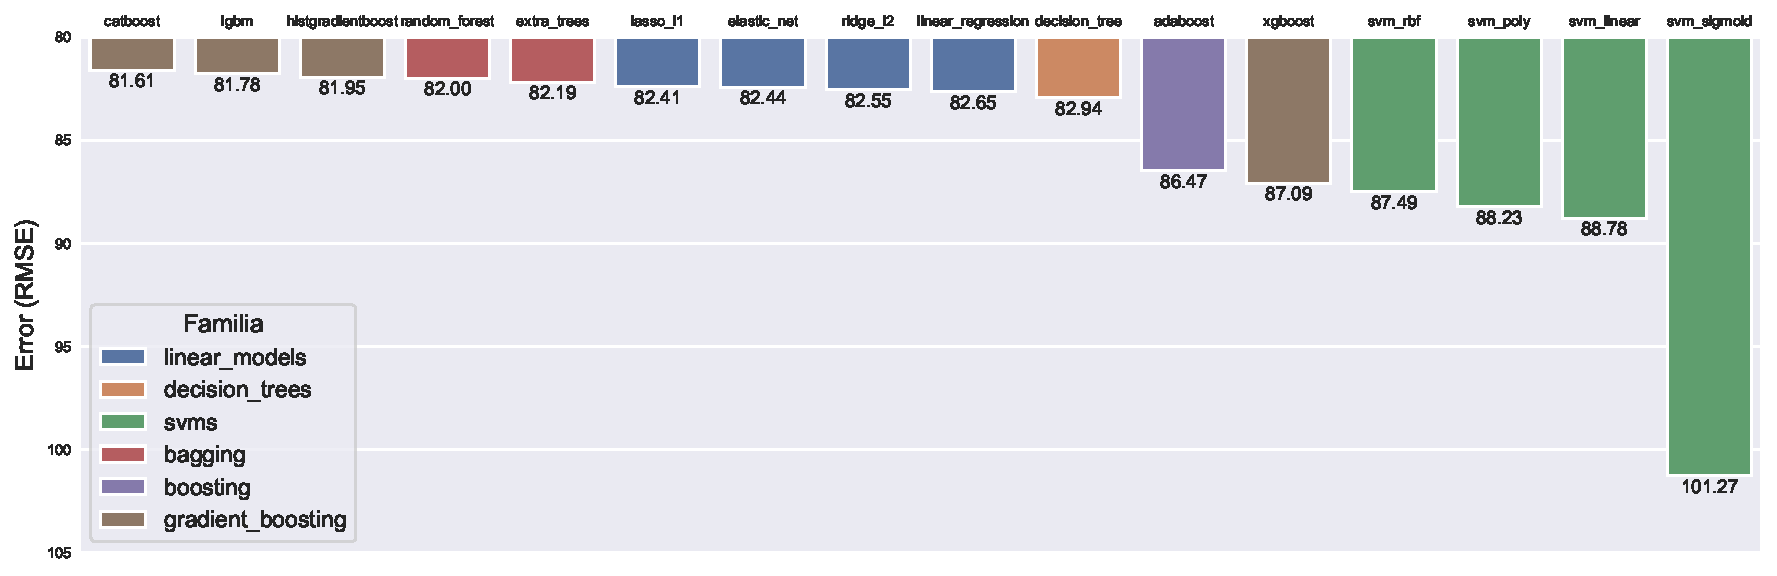
\includegraphics[width=1\linewidth]{figs/chapter5/validation/validationerror}}
	\captionsetup{belowskip=-5pt, justification=centering}
	\caption{Distribución del error de los modelos entrenados}
	\label{fig:ch5valerror}
\end{figure}

\subsection{Rendimiento del modelo final}

El último paso de la evaluación es el estudio del \textbf{rendimiento del modelo seleccionado final} - estudiando los hiperparámetros seleccionados, comprobando su \textbf{error real} sobre el conjunto de test disponible en \textit{Kaggle} y evaluando la posición hipotética que hubiera tenido durante la competición.

\subsubsection{Modelo seleccionado}

Tras el proceso de selección de modelo, el modelo de regresión seleccionado ha sido \textbf{Categorical Boost} - un \textit{ensemble de \textbf{Gradient Boosting}} utilizado como estado del arte actualmente en numerosos problemas estructurados. A través del ajuste de hiperparámetros se han seleccionado los siguientes parámetros:

\begin{itemize}[parsep=1pt, itemsep=2pt, topsep=1pt]
	\item \textbf{Subconjunto de atributos:} \textit{Filter} - \textbf{10 atributos} incluyendo los \textbf{5 atributos categóricos} seleccionados durante el análisis exploratorio de datos y \textbf{5 atributos numéricos} adicionales con información socioeconómica.
	\item \textbf{Modelos contenidos:} El \textit{ensemble} está formado por \textbf{200 árboles} (\textit{iterations}) con una profundidad máxima acotada de \textbf{8} (\textit{max\_depth}).
	\item \textbf{Ratio de aprendizaje (\textit{learning\_rate}):} $0.05$ - el aprendizaje es lento y se da poco peso a los árboles posteriores, pero sigue siendo más elevado que el valor por defecto $(0.05 > 0.03)$.
	\item \textbf{Regularización (\textit{l2\_leaf\_reg}):} $5.64$ - más elevada que el valor por defecto $(5.36>3.00)$, se penalizan los modelos complejos.
	\item \textbf{Aleatorización (\textit{random\_strength}):} $2$ - aleatoriedad añadida a los umbrales a la hora de elegir particiones para los nodos, se opta por introducir un mayor grado de aleatoriedad para tener árboles más diversos.
\end{itemize}


\subsubsection{Resultados sobre el conjunto de test y posición en la competición}

En la \textbf{Tabla \ref{tab:ch5testerror}} se puede observar el \textbf{error del modelo seleccionado} en los dos conjuntos de test disponibles: \textbf{público} (disponible durante la competición) y \textbf{privado} (mostrado tras finalizar la competición).

Además, se muestra la posición hipotética que hubiera tenido el modelo desarrollado a lo largo de este trabajo si se hubiera inscrito en la competición - junto a una comparativa del error respecto al modelo ganador de la competición y al modelo en la posición mediana.

\begin{table}[h]
	\vspace{-4mm}
	\centering
	\resizebox{0.9\textwidth}{!}{%
		\begin{tabular}{@{}ccccccc@{}}
			\toprule
			&
			&
			&
			\multicolumn{2}{c}{\textbf{Primer puesto}} &
			\multicolumn{2}{c}{\textbf{Mediana (puesto 271)}} \\ \cmidrule(l){4-7} 
			\multirow{-2}{*}{\textbf{Conjunto de test}} &
			\multirow{-2}{*}{\textbf{Error}} &
			\multirow{-2}{*}{\textbf{Posición}} &
			\textbf{Error} &
			\textbf{Diferencia} &
			\textbf{Error} &
			\textbf{Diferencia} \\ \midrule
			\multicolumn{1}{r}{\textbf{Público}} &
			\textbf{83,093} &
			249 / 542 &
			82,170 &
			+0,92 &
			83,280 &
			-0,187 \\
			\rowcolor[HTML]{EFEFEF} 
			\multicolumn{1}{r}{\cellcolor[HTML]{EFEFEF}\textbf{Privado}} &
			\textbf{81,032} &
			199 / 542 &
			80,410 &
			+0,62 &
			81,447 &
			-0,415 \\ \bottomrule
		\end{tabular}%
	}
	\captionsetup{justification=centering}
	\caption{Error del modelo seleccionado en el conjunto de test}
	\label{tab:ch5testerror}
\end{table}

A partir de esta información se puede determinar que:
\begin{itemize}[parsep=1pt, itemsep=2pt, topsep=4pt]
	\item \textbf{Sin sobreajuste:} El error del modelo se ha mantenido estable para todos los conjuntos de datos estudiados - entrenamiento, validación y test. Esto implica que no se ha sobreajustado el modelo a los datos en ningún punto, y que sus resultados son generalizables a nuevos datos.
	\item \textbf{Resultados razonables:} Si bien el modelo tiene una posición en el ranking mediocre (superior a la mediana pero lejana del primer puesto), \textbf{el error del modelo es muy cercano al del ganador de la competición} - con una diferencia inferior a 1 punto en ambos conjuntos de datos.
	\item \textbf{Error alto generalizado:} Tal y como se observó durante la selección de modelos, \textbf{el error general de los modelos es muy elevado} - siendo prácticamente equivalente a un tercio del rango de la variable objetivo, $[0,365]$.
\end{itemize}

Por todo esto, se puede afirmar que \textbf{el modelo entrenado y seleccionado es un buen predictor para el problema a resolver} - especialmente si se considera el error alto generalizado -, estando listo para ser \textbf{desplegado} a través de una aplicación.